% =============================================================================
\chapter{Results}
\label{ch:results}
% =============================================================================

Unless stated otherwise, REHAB24-6 accuracy values refer to the valid subset defined in Chapter~\ref{ch:methodology}: no detection failure, no extreme outlier above 100\% NMPJPE, and no MoCap annotation error. Inferential statements on REHAB24-6 use the subject-cluster aggregation described in Section~\ref{sec:frame-sampling}; cross-dataset comparisons with COCO are descriptive.

% -----------------------------------------------------------------------------
\section{Descriptive Statistics}
\label{sec:descriptive}
% -----------------------------------------------------------------------------

The primary three-model REHAB24-6 benchmark contains 126 processed camera-view sequences, corresponding to 367{,}200 frame-level observations before filtering, 363{,}074 after removing detection failures, and 354{,}879 in the valid central-tendency subset. Because confidence filtering and the $>$100\% outlier cut are applied per model, the valid frame counts in Table~\ref{tab:accuracy-main} differ slightly between models (115{,}711 to 119{,}729). Five c17 sequences form the coach extreme-case subset. The viewpoint distribution remains strongly bimodal after filtering: on the valid MoveNet subset, 40.8\% of frames fall into the frontal range (0--20\textdegree), 17.5\% into the intermediate range (20--60\textdegree), and 41.6\% into the lateral range (60--90\textdegree).

% -----------------------------------------------------------------------------
\section{Overall Accuracy}
\label{sec:accuracy}
% -----------------------------------------------------------------------------

Table~\ref{tab:accuracy-main} reports the primary REHAB24-6 accuracy results on the valid subset. MoveNet achieved the lowest frame-level mean NMPJPE at 10.52\%, followed by MediaPipe at 12.53\% and YOLOv8 at 12.77\%; the same ordering remained after subject-cluster aggregation.

\begin{table}[htbp]
  \centering
  \caption{Overall REHAB24-6 accuracy on the valid subset. Lower is better.}
  \label{tab:accuracy-main}
  \setlength{\tabcolsep}{3pt}
  \begin{tabular}{lcccc}
    \toprule
    Model & Mean (\%) & Median (\%) & Std (\%) & $n$ \\
    \midrule
    MoveNet   & \textbf{10.52\%} & \textbf{9.85\%} & 4.66\% & 119{,}439 \\
    MediaPipe & 12.53\% & 11.26\% & 7.05\% & 119{,}729 \\
    YOLOv8    & 12.77\% & 11.23\% & 6.73\% & 115{,}711 \\
    \bottomrule
  \end{tabular}
\end{table}

The inferential comparison uses 10 subject clusters derived from the segmentation metadata. Table~\ref{tab:accuracy-stats} shows the paired sign-flip permutation results with bootstrap confidence intervals and Holm correction. MoveNet outperformed both MediaPipe and YOLOv8 at the primary inferential level, and MediaPipe outperformed YOLOv8.

\begin{table}[htbp]
  \centering
  \caption{Pairwise REHAB24-6 accuracy comparisons on the primary subject-cluster level ($n = 10$). Differences are reported as model A minus model B in mean cluster-level NMPJPE.}
  \label{tab:accuracy-stats}
  \begin{tabular}{lcccc}
    \toprule
    Comparison & Mean difference & 95\% CI & $p$ & $p_{\mathrm{Holm}}$ \\
    \midrule
    MediaPipe $-$ MoveNet & 1.01\% & [0.62, 1.42] & 0.0020 & 0.0059 \\
    MediaPipe $-$ YOLOv8  & $-$0.49\% & [$-$0.85, $-$0.12] & 0.0352 & 0.0352 \\
    MoveNet $-$ YOLOv8    & $-$1.50\% & [$-$1.71, $-$1.27] & 0.0020 & 0.0059 \\
    \bottomrule
  \end{tabular}
\end{table}

Figure~\ref{fig:accuracy-boxplot} shows the per-cluster distribution that underlies this test. The separation between MoveNet and the two alternatives is visible across most clusters, whereas MediaPipe and YOLOv8 show more overlap.

\begin{figure}[htbp]
  \centering
  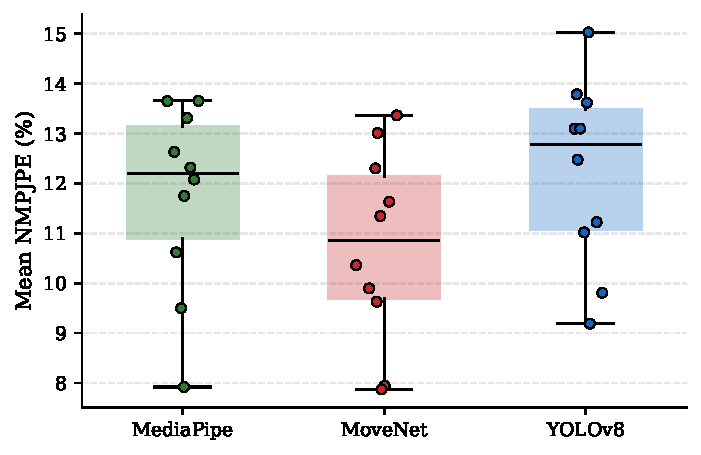
\includegraphics[width=0.9\textwidth]{fig/fig_accuracy_boxplot.pdf}
  \caption{Subject-cluster accuracy distributions on REHAB24-6. Each point represents one subject cluster defined by the segmentation metadata; boxplots summarize the distribution of the cluster-level mean of per-video median NMPJPE across the 10 clusters. Lower is better.}
  \label{fig:accuracy-boxplot}
\end{figure}

Per-exercise aggregation confirms that MoveNet ranks first on all six REHAB24-6 exercises (Appendix~\ref{app:per-exercise}).

% -----------------------------------------------------------------------------
\section{Model Variants}
\label{sec:variant-results}
% -----------------------------------------------------------------------------

Table~\ref{tab:variant-accuracy} extends the REHAB24-6 comparison to all nine model variants. MoveNet MultiPose achieved the lowest valid-subset NMPJPE. Within families, larger YOLOv8 variants improved over Nano, MediaPipe Heavy improved over Full and Lite, MoveNet SP\_Lightning traded accuracy for a substantial speed gain, and MoveNet SP\_Thunder traded accuracy without a meaningful speed advantage over MultiPose.

\begin{table}[htbp]
  \centering
  \caption{REHAB24-6 valid-subset accuracy for all nine evaluated variants. Lower is better.}
  \label{tab:variant-accuracy}
  \begin{tabular}{lccc}
    \toprule
    Variant & Mean NMPJPE & Median NMPJPE & Valid frames \\
    \midrule
    MoveNet\_MultiPose     & \textbf{10.52\%} & \textbf{9.85\%} & 119{,}439 \\
    YOLOv8\_Medium         & 10.86\% & 10.01\% & 114{,}591 \\
    YOLOv8\_Small          & 11.43\% & 10.27\% & 116{,}009 \\
    MediaPipe\_Heavy       & 11.51\% & 10.59\% & 119{,}630 \\
    MediaPipe\_Full        & 12.53\% & 11.26\% & 119{,}729 \\
    YOLOv8\_Nano           & 12.77\% & 11.23\% & 115{,}711 \\
    MoveNet\_SP\_Thunder   & 13.33\% & 11.93\% & 117{,}719 \\
    MediaPipe\_Lite        & 13.54\% & 11.77\% & 119{,}392 \\
    MoveNet\_SP\_Lightning & 14.97\% & 12.83\% & 94{,}395 \\
    \bottomrule
  \end{tabular}
\end{table}

% -----------------------------------------------------------------------------
\section{Cross-Dataset Comparison}
\label{sec:crossdataset-results}
% -----------------------------------------------------------------------------

Table~\ref{tab:crossdataset} compares the variant rankings between REHAB24-6 and COCO val2017. On REHAB24-6, MoveNet MultiPose ranked first, whereas YOLOv8 Medium ranked first on COCO. When COCO is restricted to single-person images, the leading order of the strongest COCO variants is preserved and the ranking shift relative to REHAB24-6 persists.

\begin{table}[htbp]
  \centering
  \small
  \caption{Cross-dataset ranking comparison for all nine variants. ``COCO single'' refers to the valid subset restricted to images containing one annotated person.}
  \label{tab:crossdataset}
  \setlength{\tabcolsep}{4pt}
  \begin{tabular}{lccccc}
    \toprule
    Variant & REHAB rk.\ & REHAB \% & COCO rk.\ & COCO \% & COCO single \% \\
    \midrule
    MoveNet\_MultiPose     & 1 & 10.52\% & 4 & 12.44\% & 12.55\% \\
    YOLOv8\_Medium         & 2 & 10.86\% & 1 & 10.15\% & 10.53\% \\
    YOLOv8\_Small          & 3 & 11.43\% & 2 & 10.88\% & 11.74\% \\
    MediaPipe\_Heavy       & 4 & 11.51\% & 7 & 15.08\% & 14.50\% \\
    MediaPipe\_Full        & 5 & 12.53\% & 8 & 17.21\% & 16.73\% \\
    YOLOv8\_Nano           & 6 & 12.77\% & 6 & 13.69\% & 14.87\% \\
    MoveNet\_SP\_Thunder   & 7 & 13.33\% & 3 & 12.01\% & 11.84\% \\
    MediaPipe\_Lite        & 8 & 13.54\% & 9 & 20.07\% & 19.33\% \\
    MoveNet\_SP\_Lightning & 9 & 14.97\% & 5 & 12.63\% & 12.61\% \\
    \bottomrule
  \end{tabular}
\end{table}

Figure~\ref{fig:crossdataset-slopegraph} visualizes these rank movements directly. The largest shifts affect the MoveNet family and the larger MediaPipe variants, while YOLOv8 changes least overall.

\begin{figure}[htbp]
  \centering
  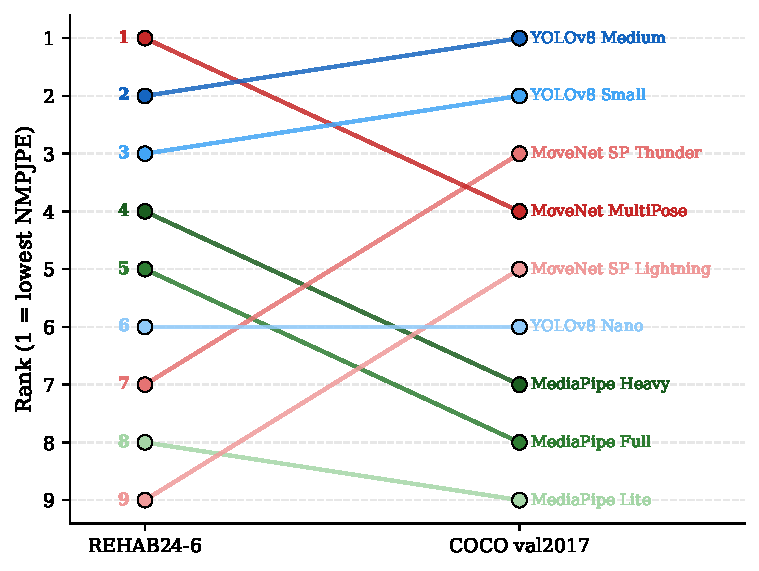
\includegraphics[width=\textwidth]{fig/fig_cross_dataset_slopegraph.pdf}
  \caption{Ranking shifts between REHAB24-6 and COCO val2017 across the nine evaluated variants. Rankings are based on mean NMPJPE within each dataset's valid subset, with rank~1 indicating the lowest NMPJPE. Exact mean values are reported in Table~\ref{tab:crossdataset}.}
  \label{fig:crossdataset-slopegraph}
\end{figure}

Among the three main models, MoveNet ranked first on both datasets, while YOLOv8 and MediaPipe swapped order.

% -----------------------------------------------------------------------------
\section{Viewpoint Sensitivity}
\label{sec:rotation-results}
% -----------------------------------------------------------------------------

Table~\ref{tab:rotation} summarizes the frontal-to-lateral viewpoint degradation on REHAB24-6. MoveNet exhibited the smallest increase from frontal to lateral views (+17.8\%), followed by MediaPipe (+27.5\%) and YOLOv8 (+31.7\%).

\begin{table}[htbp]
  \centering
  \caption{REHAB24-6 viewpoint sensitivity on the valid subset. Frontal corresponds to 0--20\textdegree{} and lateral to 60--90\textdegree{}.}
  \label{tab:rotation}
  \begin{tabular}{lccc}
    \toprule
    Model & Frontal mean & Lateral mean & Degradation \\
    \midrule
    MoveNet   & \textbf{9.75\%} & \textbf{11.49\%} & \textbf{+17.8\%} \\
    MediaPipe & 11.28\% & 14.38\% & +27.5\% \\
    YOLOv8    & 11.14\% & 14.66\% & +31.7\% \\
    \bottomrule
  \end{tabular}
\end{table}

Figure~\ref{fig:rotation-line} shows the full binned trend across 10\textdegree{} rotation bins. The uneven pattern in the intermediate bins reflects the fixed-camera geometry and strongly bimodal viewpoint distribution; the figure should not be read as a densely sampled continuous rotation study.

\begin{figure}[htbp]
  \centering
  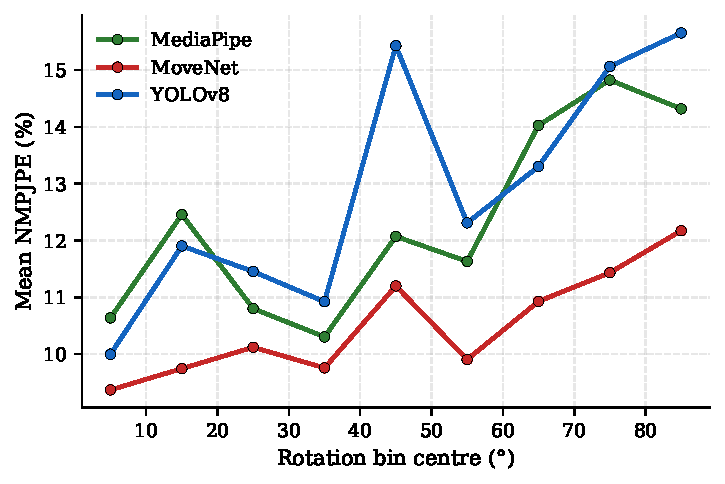
\includegraphics[width=\textwidth]{fig/fig_rotation_line.pdf}
  \caption{Mean NMPJPE by 10\textdegree{} rotation bin on the REHAB24-6 valid subset. Points show binned means; the connecting lines visualize the viewpoint trend across bins. Under REHAB24-6's fixed camera geometry and bimodal viewpoint distribution, this figure should be interpreted as a viewpoint comparison rather than as a dense continuous rotation study. Lower is better.}
  \label{fig:rotation-line}
\end{figure}

% -----------------------------------------------------------------------------
\section{Multi-Person Behavior}
\label{sec:multiperson-results}
% -----------------------------------------------------------------------------

We analyze multi-person behavior in two subsets: a segmentation-defined subset covering the full benchmark and an extreme-case coach subset of five c17 views with a prominently visible therapist.

\paragraph{Segmentation-defined subset.}
On the segmentation-based multi-person subset, the filtered mean error changed only slightly relative to the remaining valid frames. MediaPipe increased by 1.2\%, while MoveNet and YOLOv8 were slightly lower on the multi-person subset than on the complementary subset.

\begin{table}[htbp]
  \centering
  \caption{REHAB24-6 segmentation-defined multi-person subset (severity $\geq 2$) on the valid data.}
  \label{tab:multiperson}
  \begin{tabular}{lcccc}
    \toprule
    Model & Single-person mean & Multi-person mean & Change & Multi-person frames \\
    \midrule
    MediaPipe & 12.51\% & 12.67\% & +1.2\% & 10{,}596 \\
    MoveNet   & \textbf{10.56\%} & \textbf{10.04\%} & $-$5.0\% & 10{,}703 \\
    YOLOv8    & 12.82\% & 12.25\% & $-$4.4\% & 10{,}286 \\
    \bottomrule
  \end{tabular}
\end{table}

\paragraph{Coach extreme-case subset.}
The five coach sequences show a different failure regime. Table~\ref{tab:coach-detection} combines the raw detection-count analysis with the catastrophic outlier rate on the coach subset. MediaPipe detected two or more persons in 23\% of sampled coach frames, MoveNet in 16\%, and YOLOv8 in 62\%; the corresponding coach-scene outlier rates were 9.1\%, 13.8\%, and 13.9\%.

\begin{table}[htbp]
  \centering
  \caption{Coach extreme-case subset: sampled secondary-person frequency, coach-scene outlier rate, and mean NMPJPE. Detection counts are based on every tenth frame across 1{,}178 sampled coach frames; outlier rates and mean NMPJPE are computed over all non-failure coach frames, with NMPJPE reported before the $>$100\% outlier cut so that catastrophic misassignment events remain reflected in the mean.}
  \label{tab:coach-detection}
  \begin{tabular}{lccc}
    \toprule
    Model & 2+ persons detected & Coach outlier rate & Mean coach NMPJPE \\
    \midrule
    MediaPipe & 23\% & \textbf{9.1\%} & \textbf{45.4\%} \\
    MoveNet   & 16\% & 13.8\% & 62.2\% \\
    YOLOv8    & 62\% & 13.9\% & 66.0\% \\
    \bottomrule
  \end{tabular}
\end{table}

The five coach videos differ substantially. Table~\ref{tab:coach-detail} shows that PM\_010-c17 is the only coach sequence in which all three models exhibit sequence-level mean NMPJPE above 65\%, whereas MediaPipe stays below 40\% in the other four coach sequences.

\begin{table}[htbp]
  \centering
  \caption{Per-video mean NMPJPE on the five coach extreme-case sequences.}
  \label{tab:coach-detail}
  \begin{tabular}{lccc}
    \toprule
    Coach sequence & MediaPipe & MoveNet & YOLOv8 \\
    \midrule
    PM\_010-c17 & 81.9\% & 70.7\% & 69.9\% \\
    PM\_011-c17 & 38.0\% & 59.7\% & 66.2\% \\
    PM\_108-c17 & 17.2\% & 46.2\% & 51.1\% \\
    PM\_119-c17 & 24.1\% & 74.0\% & 73.0\% \\
    PM\_121-c17 & 30.9\% & 60.3\% & 75.3\% \\
    \bottomrule
  \end{tabular}
\end{table}

Figure~\ref{fig:coach-detection-comparison} illustrates the distinct model outputs on a coach extreme-case frame.

\begin{figure}[htbp]
  \centering
  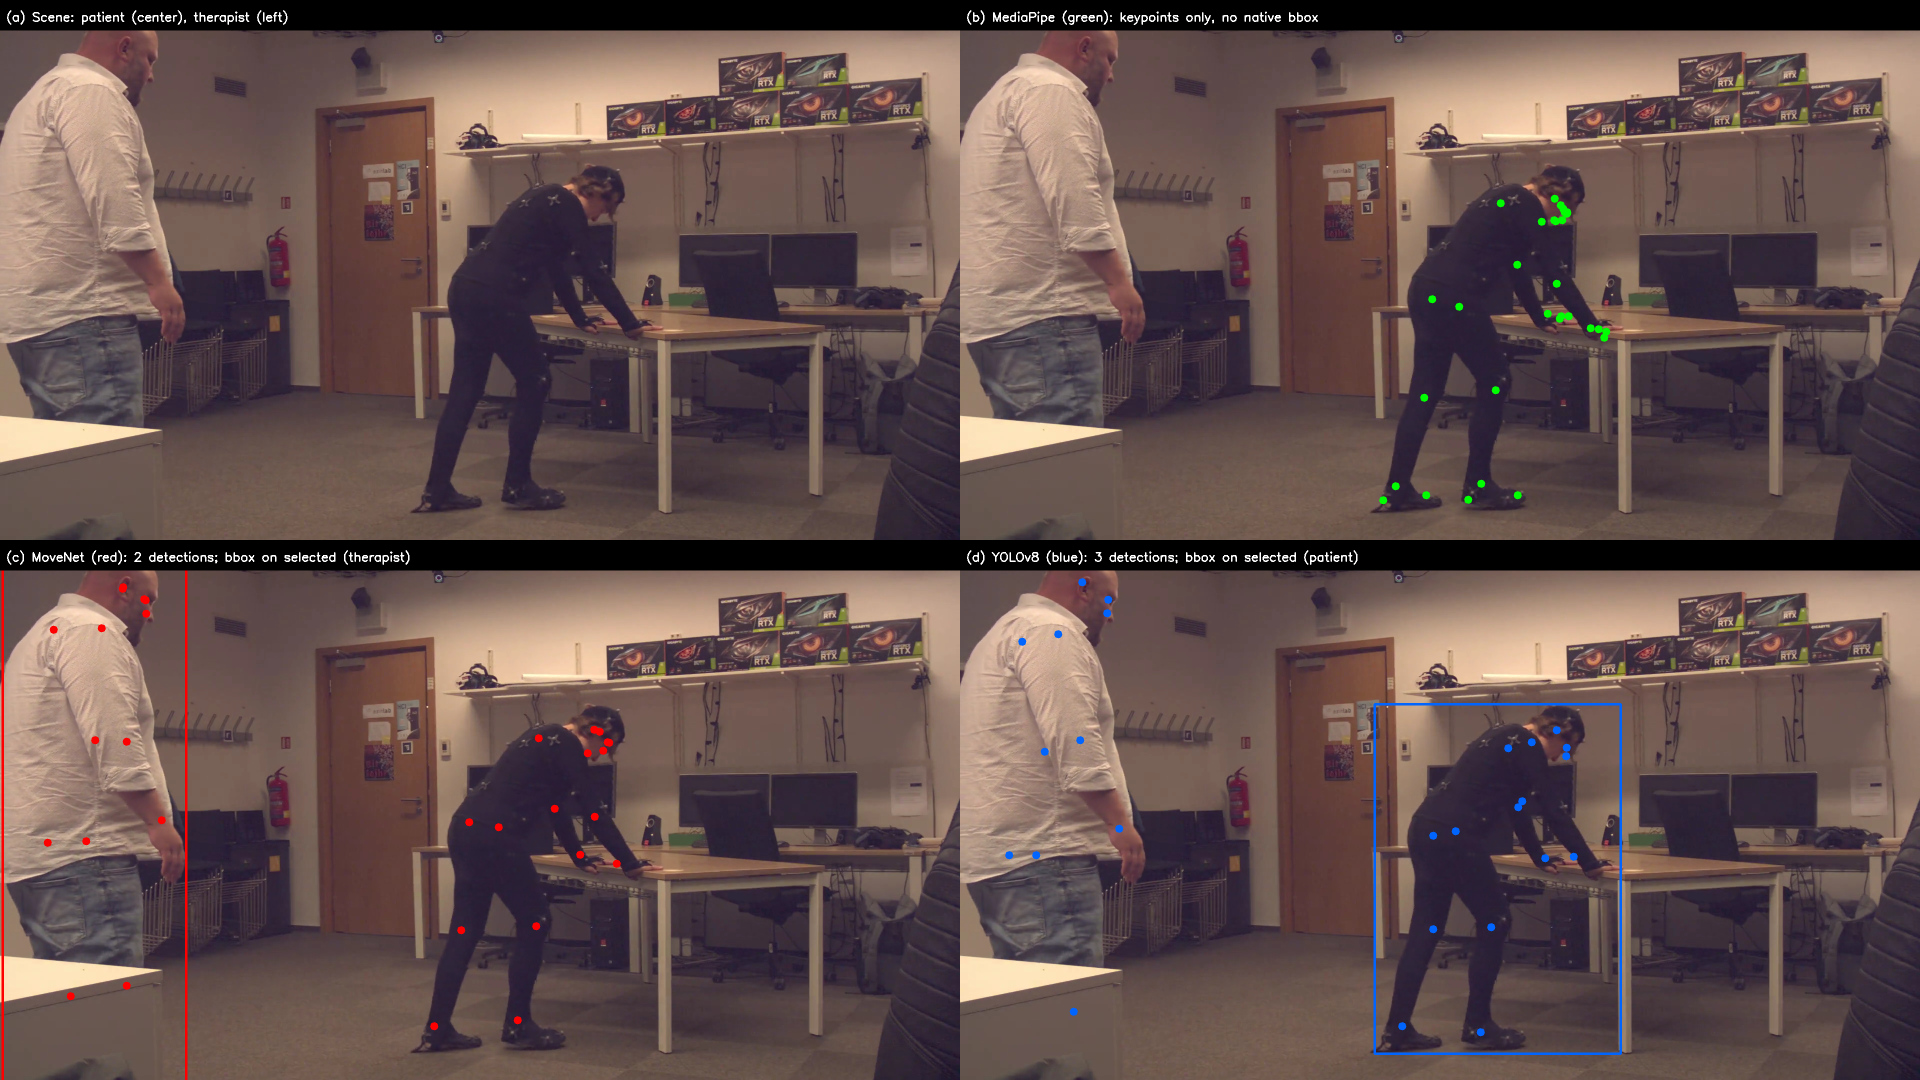
\includegraphics[width=\textwidth]{fig/coach_detection_comparison.png}
  \caption{Illustrative outputs on a coach extreme-case frame (PM\_119-c17, frame 105). MediaPipe (green) localizes the patient; MoveNet (red) detects patient and therapist but selects the therapist under the largest-area rule; YOLOv8 (blue) detects patient, therapist, and a partial border person but selects the patient. Keypoints are shown for all detections; native bounding boxes are drawn only for the selected candidate. Aggregate coach-scene frequencies are reported in Table~\ref{tab:coach-detection}.}
  \label{fig:coach-detection-comparison}
\end{figure}

% -----------------------------------------------------------------------------
\section{Temporal Stability}
\label{sec:stability-results}
% -----------------------------------------------------------------------------

Temporal stability is assessed through normalized frame-to-frame prediction displacement on valid frame pairs. MoveNet produced the lowest mean displacement at 3.81\%, followed by YOLOv8 at 5.22\% and MediaPipe at 6.03\%.

Across all nine variants, the lowest mean displacement was observed for MoveNet\_SP\_Thunder (3.31\%), followed by MoveNet\_SP\_Lightning (3.61\%) and MoveNet\_MultiPose (3.81\%).

% -----------------------------------------------------------------------------
\section{Detection Completeness}
\label{sec:detection-results}
% -----------------------------------------------------------------------------

Table~\ref{tab:detection} summarizes detection completeness. YOLOv8 produced full 12-joint detections in 79.1\% of frames, compared to 55.1\% for MediaPipe and 38.2\% for MoveNet.

\begin{table}[htbp]
  \centering
  \caption{Detection completeness on REHAB24-6 after removing full-frame detection failures.}
  \label{tab:detection}
  \begin{tabular}{lccc}
    \toprule
    Model & Full detection (12/12) & Mean valid joints & Median valid joints \\
    \midrule
    MediaPipe & 55.1\% & 10.72 & 12 \\
    MoveNet   & 38.2\% & 10.31 & 11 \\
    YOLOv8    & \textbf{79.1\%} & \textbf{11.53} & \textbf{12} \\
    \bottomrule
  \end{tabular}
\end{table}

% -----------------------------------------------------------------------------
\section{Inference Time and Speed--Accuracy Trade-offs}
\label{sec:inference-results}
% -----------------------------------------------------------------------------

Table~\ref{tab:inference} reports the CPU-only inference benchmark for all nine evaluated variants. MoveNet\_SP\_Lightning was the fastest configuration at 100.6\,FPS, whereas YOLOv8\_Medium was the slowest at 4.6\,FPS.

\begin{table}[htbp]
  \centering
  \caption{CPU-only inference benchmark for all nine evaluated variants.}
  \label{tab:inference}
  \begin{tabular}{lcccc}
    \toprule
    Variant & Mean (ms) & Median (ms) & FPS & P95 (ms) \\
    \midrule
    MoveNet\_SP\_Lightning & \textbf{9.9} & \textbf{9.8} & \textbf{100.6} & 10.9 \\
    MoveNet\_MultiPose     & 36.1 & 34.8 & 27.7 & 45.8 \\
    MoveNet\_SP\_Thunder   & 36.2 & 36.0 & 27.6 & 38.1 \\
    MediaPipe\_Lite        & 45.7 & 42.2 & 21.9 & 70.9 \\
    YOLOv8\_Nano           & 52.9 & 51.1 & 18.9 & 60.3 \\
    MediaPipe\_Full        & 67.9 & 64.0 & 14.7 & 116.1 \\
    YOLOv8\_Small          & 97.1 & 93.9 & 10.3 & 107.5 \\
    MediaPipe\_Heavy       & 165.3 & 135.3 & 6.0 & 304.1 \\
    YOLOv8\_Medium         & 215.4 & 211.1 & 4.6 & 246.3 \\
    \bottomrule
  \end{tabular}
\end{table}

Figure~\ref{fig:speed-accuracy-scatter} combines REHAB24-6 valid-subset accuracy with the dedicated sequential CPU benchmark. The dashed frontier marks the non-dominated configurations under these two criteria.

\begin{figure}[htbp]
  \centering
  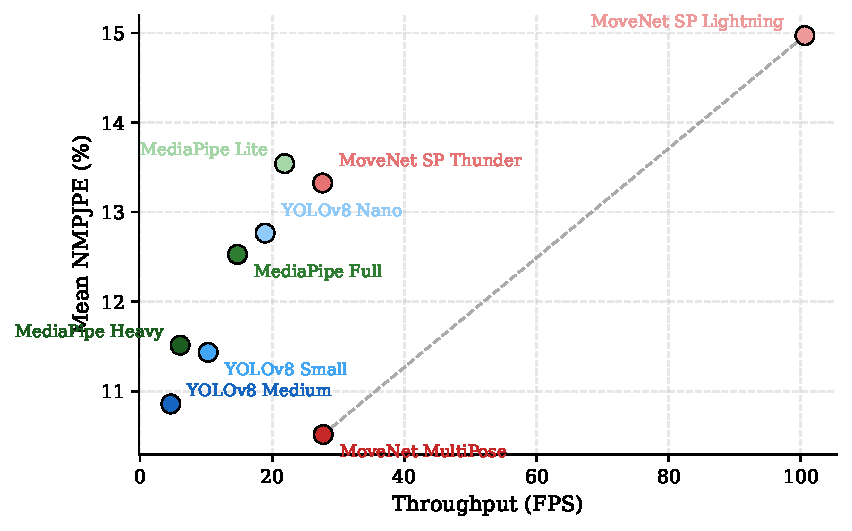
\includegraphics[width=\textwidth]{fig/fig_speed_accuracy_scatter.pdf}
  \caption{Speed--accuracy trade-off across all nine evaluated variants. The horizontal axis shows throughput from the dedicated sequential CPU-only inference benchmark; the vertical axis shows mean NMPJPE on the REHAB24-6 valid subset. The dashed line marks the non-dominated configurations under these two criteria. Lower and further right is better.}
  \label{fig:speed-accuracy-scatter}
\end{figure}

Figure~\ref{fig:speed-accuracy-scatter} together with Tables~\ref{tab:variant-accuracy} and~\ref{tab:inference} shows that several family-level accuracy gains come at substantial latency cost, most clearly for MediaPipe Heavy and YOLOv8 Medium.

The reported throughput reflects the implemented native deployment stacks as well as the model variants themselves, not a backend-normalized architecture benchmark.

% -----------------------------------------------------------------------------
\section{Per-Joint Error Patterns}
\label{sec:perjoint-results}
% -----------------------------------------------------------------------------

Table~\ref{tab:perjoint} summarizes the regional error profile across the 12 evaluated joints. MediaPipe shows the highest hip error among the three main models, while MoveNet yields the lowest error in the lower-body regions overall.

\begin{table}[htbp]
  \centering
  \caption{Regional per-joint NMPJPE on the REHAB24-6 valid subset.}
  \label{tab:perjoint}
  \begin{tabular}{lccc}
    \toprule
    Body region & MediaPipe & MoveNet & YOLOv8 \\
    \midrule
    Shoulders & \textbf{8.76\%} & 10.29\% & 10.21\% \\
    Elbows    & 11.24\% & \textbf{10.00\%} & 13.08\% \\
    Wrists    & 12.01\% & \textbf{11.84\%} & 16.25\% \\
    Hips      & 16.72\% & \textbf{11.28\%} & 14.59\% \\
    Knees     & 9.92\% & \textbf{7.76\%} & 9.87\% \\
    Ankles    & 14.59\% & \textbf{11.41\%} & 12.59\% \\
    \bottomrule
  \end{tabular}
\end{table}

On the three main models, MediaPipe's mean NMPJPE decreases from 12.53\% to 11.66\% when the hip joints are excluded, whereas MoveNet changes only marginally from 10.52\% to 10.46\%. The MediaPipe--MoveNet gap shrinks from 2.01 percentage points on all 12 joints to 1.21 percentage points on the 10 non-hip joints.

% -----------------------------------------------------------------------------
\section{Failure-Mode Decomposition}
\label{sec:failure-modes}
% -----------------------------------------------------------------------------

The previous sections report separate failure indicators---detection failures, high-NMPJPE outliers, multi-person context, low valid-joint counts. We combine them into one mutually exclusive taxonomy that classifies every failure frame into one of four categories. A frame counts as a failure if it is flagged as a detection failure or as an NMPJPE outlier (${>}100\%$ of torso length). The four categories are applied in order:

\begin{enumerate}
  \item \textbf{Missing-Detection}: the model returned no detection for the frame.
  \item \textbf{Confidence-Collapse}: detection succeeded, but fewer than six of the 12 evaluated joints remained after the joint-level confidence filter.
  \item \textbf{Multi-Person-Confusion}: outlier with sufficient valid joints in a frame with a visible secondary person (\texttt{extra\_person\_severity} $\geq 2$).
  \item \textbf{Keypoint-Displacement}: outlier with sufficient valid joints in a frame without a clearly visible secondary person---a catastrophic misprediction without an obvious detection- or selection-level cause.
\end{enumerate}

\begin{figure}[htbp]
  \centering
  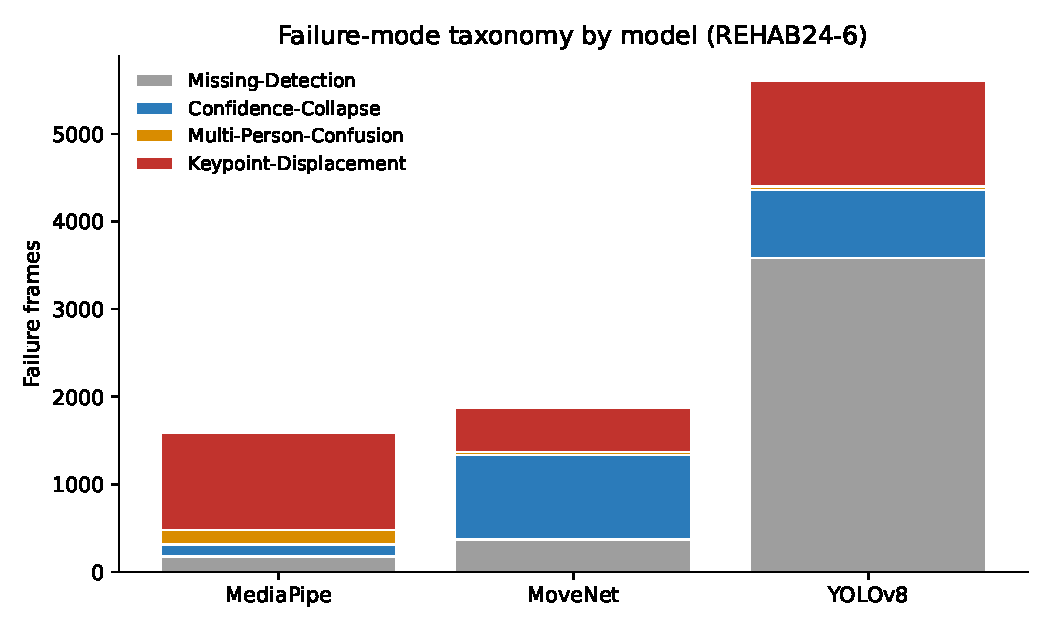
\includegraphics[width=0.85\textwidth]{fig/failure_mode_taxonomy.pdf}
  \caption{Failure-mode distribution on REHAB24-6. Each bar represents one main model; the four segments give the absolute number of failure frames per category. Exact counts are reported in Table~\ref{tab:failure-mode-counts}.}
  \label{fig:failure-modes}
\end{figure}

Each model is dominated by a different category. MediaPipe failures are predominantly Keypoint-Displacement (69.6\% of 1{,}583 failures), MoveNet failures are predominantly Confidence-Collapse (51.4\% of 1{,}875), and YOLOv8 has the largest absolute failure count, driven by Missing-Detection (63.8\% of 5{,}610). YOLOv8 returned no prediction for 3{,}580 frames, roughly twenty times the MediaPipe rate. Multi-Person-Confusion accounts for at most 11\% of failures across models.

The split is robust to the Confidence-Collapse threshold. Varying the valid-joint cutoff between 4 and 8 preserves the dominant category for each model.
